\section{Background}\label{sec:background}

\subsection{Software that only grows}\label{sec:decay}

That software decays when it only accumulates features is one of the oldest
observations in software engineering. Lehman's laws of software evolution hold that a
program in real-world use must keep changing, and that its complexity grows as
it evolves unless work is done to maintain or reduce it~\cite{lehman1980laws};
a later formulation adds that its quality will appear to decline unless it is
rigorously maintained and adapted~\cite{lehman1997metrics}. Parnas called the
result software aging, and blamed in part the changes made by people who do
not understand the original design~\cite{parnas1994aging}. Eick and colleagues
found mixed but, on the whole, persuasive evidence of code decay in fifteen-plus
years of change data from a large telephone-switching
system~\cite{eick2001decay}. Cunningham's technical-debt metaphor framed the
cost of not consolidating as interest paid on every later
change~\cite{cunningham1992wycash}, and Fowler's design stamina hypothesis
holds that without attention to design, adding features eventually becomes
slower than it would have been with it~\cite{fowler2007stamina}. Studies have
since put numbers on the interest: across 39 proprietary code bases,
low-quality files had fifteen times more defects and their issues took
124\% longer to resolve in a CodeScene-associated vendor
study~\cite{tornhill2022codered}; 43 developers self-reported losing about
23\% of their working time to technical debt in a longitudinal
study~\cite{besker2018cripples}. These are different outcomes and populations.

The evidence is not universal. Increasing complexity and declining quality
are among the less strongly supported of Lehman's laws, and some systems have
grown without the predicted decay~\cite{herraiz2013laws}. Several findings
above are observational, and their estimates belong to the studied settings,
not every code base.

The engineering intuition often called \emph{software entropy} is that keeping
a changing system coherent requires counter-work: removing obsolete paths,
restoring boundaries and revisiting assumptions. Software does not deteriorate
simply because time passes, and thermodynamic entropy supplies no measure of
its quality. Here the measurable quantities are losses of required behaviour,
excess structural burden and the effort needed for a later change.

\subsection{What carries from one feature to the next?}\label{sec:inheritance}

Feature accumulation is the addition of capabilities and interactions; churn
is the editing activity that implements, replaces or removes them. Neither
is itself deterioration. A \emph{regression} loses previously working
behaviour that is still required. A never-implemented feature is instead an
acquisition failure. Persistence means that the same fault remains unresolved;
propagation means that a later, distinct fault or failure can be traced to
reuse of the earlier one. \emph{Compounding} is the stronger claim that the
earlier error increases subsequent error risk or change burden.

These distinctions matter because an agent inherits more than a code diff.
The repository supplies implementations, tests, interfaces and deployment
assumptions. Instructions, skills and notes supply an account of how to work
on them. A mistaken rule can become code, then a test expectation or an
instruction, and finally the precedent used for another feature. The stored
record need not be correct to become authoritative in the next session.
Conversely, an inherited implementation can be sound even when it differs
from a human reference. The question is what subsequent work can achieve
from that state.

\begin{figure}[!htbp]
\centering
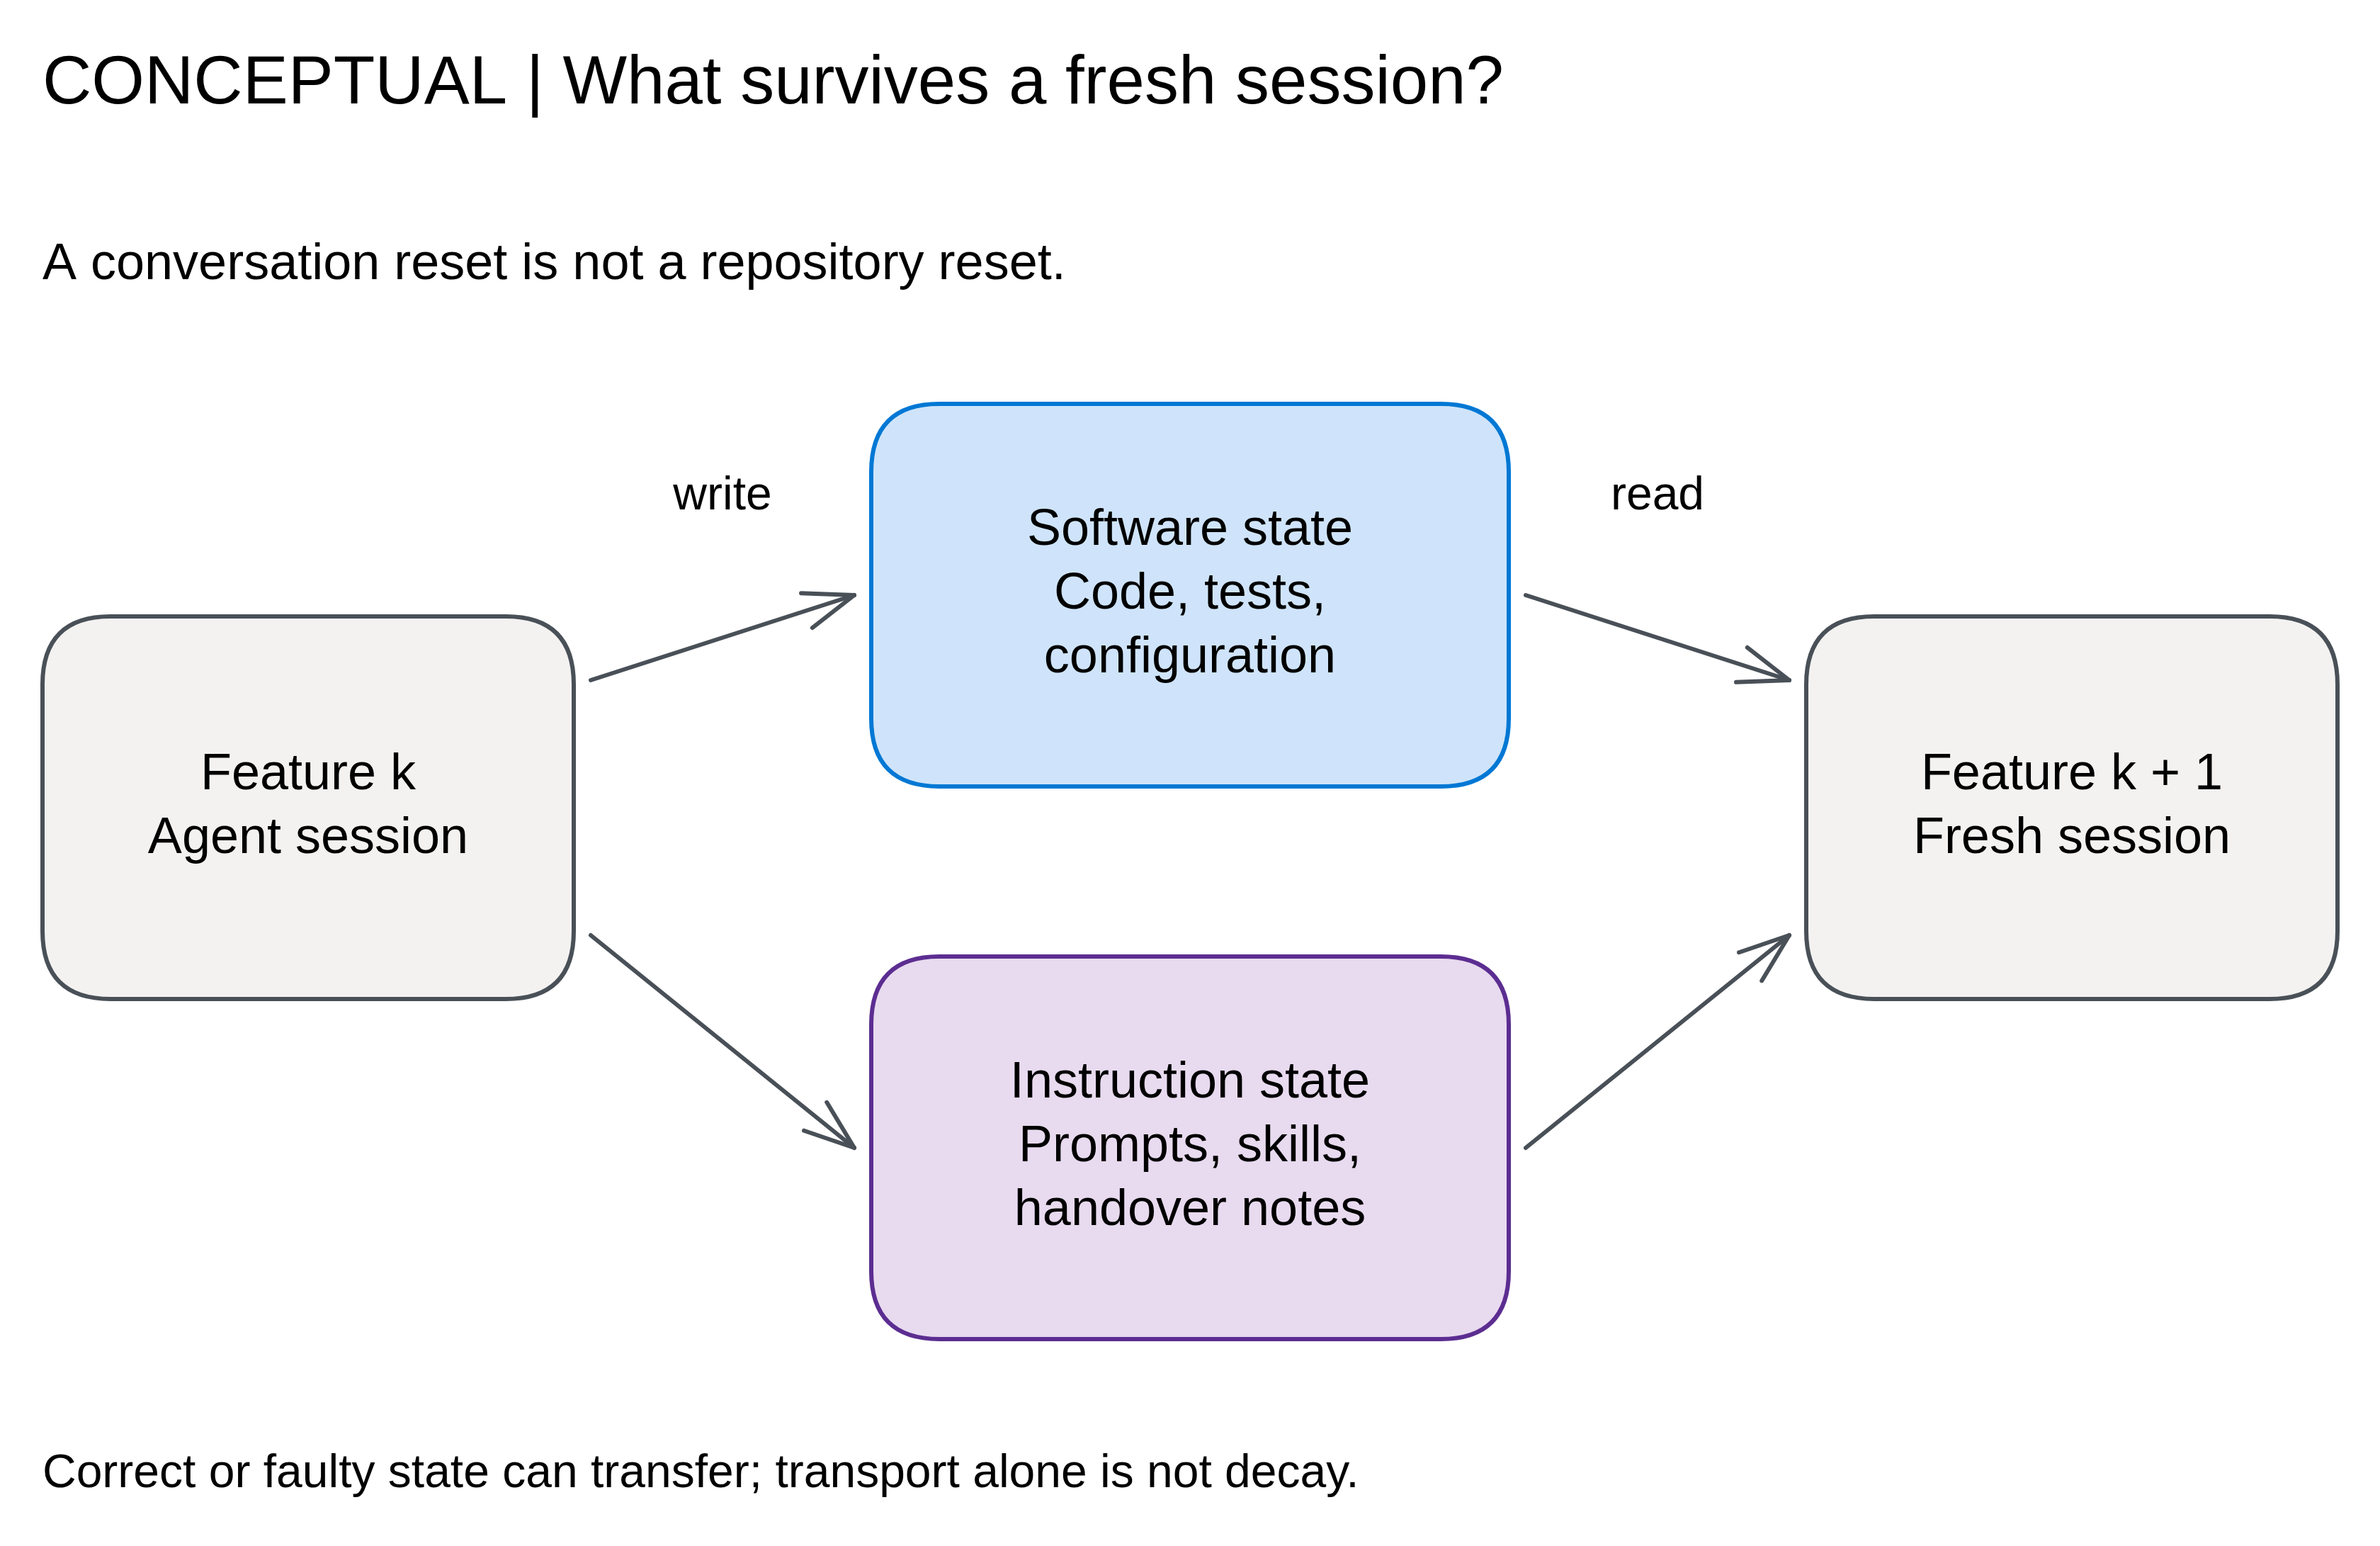
\includegraphics[width=\linewidth]{fig-state-inheritance.png}
\caption{Conceptual state transfer between feature sessions. A fresh
conversation does not reset inherited software or instruction state.
Solid arrows denote possible read/write paths, not measured error
propagation. Both channels can carry correct decisions as well as faults;
their presence alone is not evidence of decay.}\label{fig:stateinheritance}
\end{figure}

Figure~\ref{fig:stateinheritance} separates the two persistent channels from
conversation history. It is an explanatory model, not an observed trajectory
or a claim that every tool retains the same material.

\subsection{Compounding within and between features}\label{sec:empirical}

\paragraph{Errors carried in conversation.}
An earlier answer changes the context from which a model produces the next
one. Experiments on this pathway distinguish dependence on an erroneous
history from the difficulty of a long task.

Zhang et~al.'s earlier \emph{How Language Model Hallucinations Can Snowball}
shows why consistency is not enough. On three question-answering datasets,
ChatGPT and GPT-4 produce false justifications after wrong answers, yet often
reject the individual false claims when questioned in a separate session.
Their explanation is over-commitment to the earlier answer rather than only
a lack of knowledge. The inspected original experiments concern question answering in two
2023 models; the later ICML publication expands the model coverage
~\cite[original preprint, Secs.~3.1--3.4]{zhang2023snowball}.

Sinha et~al. test the distinction directly in a controlled execution task.
Models receive both the lookup dictionary and the plan, then maintain a
running sum. The authors vary the fraction of incorrect answers in artificial
prior histories and measure the accuracy of subsequent state updates, not
merely whether the final total remains correct. More erroneous history reduces
later accuracy beyond the effect of context length. This is counterfactual
evidence of \emph{self-conditioning}: earlier mistakes can increase the chance
of new mistakes. Scaling non-thinking models does not remove the effect, but
Qwen3 models with thinking enabled avoid it in this setup. The result identifies
a dependence on model configuration as well as erroneous history
\cite[Secs.~2.2--3, Figs.~5--6]{sinha2025illusion}.

Laban et~al. supply complementary conversational evidence. Across six
generation tasks, including Python and SQL, they report a 39\% average relative
performance drop when instructions arrive through underspecified multi-turn
conversation rather than all at once. A concatenated-instruction control
largely preserves performance, weakening information loss from rephrasing as
the explanation. Their analyses associate premature answers with lower success
and describe reliance on earlier incorrect attempts and increasingly bloated
solutions. These are simulated conversations and diagnostic analyses, not a
controlled estimate of the cost of a particular inherited coding defect; the
39\% is not a percentage-point loss or a repository defect
rate~\cite[arXiv v1, Secs.~3.3 and~6.1, App.~F.1--F.2]{laban2025lost}.

\paragraph{Errors carried in the repository.}
Pan et~al.'s \emph{SWE-Maintain} preprint tests the pathway most directly
relevant to successive feature work. It reconstructs 100 three-event
maintenance episodes from 50 Python
repositories and runs each later task from two starting points: the developers'
preceding patches and the agent's own preceding changes. Task, agent and tests
are held fixed, and every event uses a fresh session: only the repository
carries the earlier work forward. Across 1,996 paired later events, agent
history lowers new-task resolution by 5.6 percentage points (95\% interval
$[-7.2,-4.1]$). Requiring earlier tests to remain passing widens the gap to
14.0 points. The unweighted mean new-task gap grows from 4.0 points at the second
event to 7.2 at the third, consistent with an accumulating downstream cost,
though three-event episodes cannot establish a general long-horizon decay
law~\cite[Secs.~2.5 and~4.1, Table~2]{pan2026swemaintain}.

Their \texttt{python\_unidiff} example makes the proposed propagation concrete:
an agent splits a string into lines, losing line terminators; the next
task reuses that logic in a constructor, while developer history succeeds.
The framing appears in Figure~1's caption and the detailed failure in
Section~5.1 and Figure~5~\cite{pan2026swemaintain}.
Their \texttt{parse\_crontab} example exposes a less visible dependency:
an agent's local Python~3 fix passes the current and next tests, but later
code relies on module-wide compatibility aliases that it never supplied.
The later compatibility failure is discussed in
Section~5.1 and Figure~5~\cite{pan2026swemaintain}.
Among the 619 later events
whose inherited code passes earlier tests and whose next task is not already
solved, the new-task-only difference is $-1.1$ points (95\% interval
$[-3.8,+1.6]$), and the event-resolution difference is $+2.7$ points (95\% interval
$[-0.5,+6.1]$), with no detected disadvantage. This is a selected clean-history
subset, not a randomised repair intervention, and it does not prove equivalent
maintainability under all changes. It points more directly to inherited
behavioural failures than to structural complexity as the main observed
channel~\cite[Sec.~4.2, Table~3; Sec.~5.1, Fig.~5]{pan2026swemaintain}.

Figure~\ref{fig:inheritedhistory} shows the published event-resolution
contrasts, including the clean-history cohorts. Event resolution requires
the new task and all earlier non-superseded tests to pass. Its larger gap
therefore includes retained failures as well as difficulty solving the new
task. The current-task-only difference of $-5.6$ points is important for the
cross-feature hypothesis precisely because it does not count earlier failing
tests against success on the new task.

\begin{figure}[!htbp]
\centering
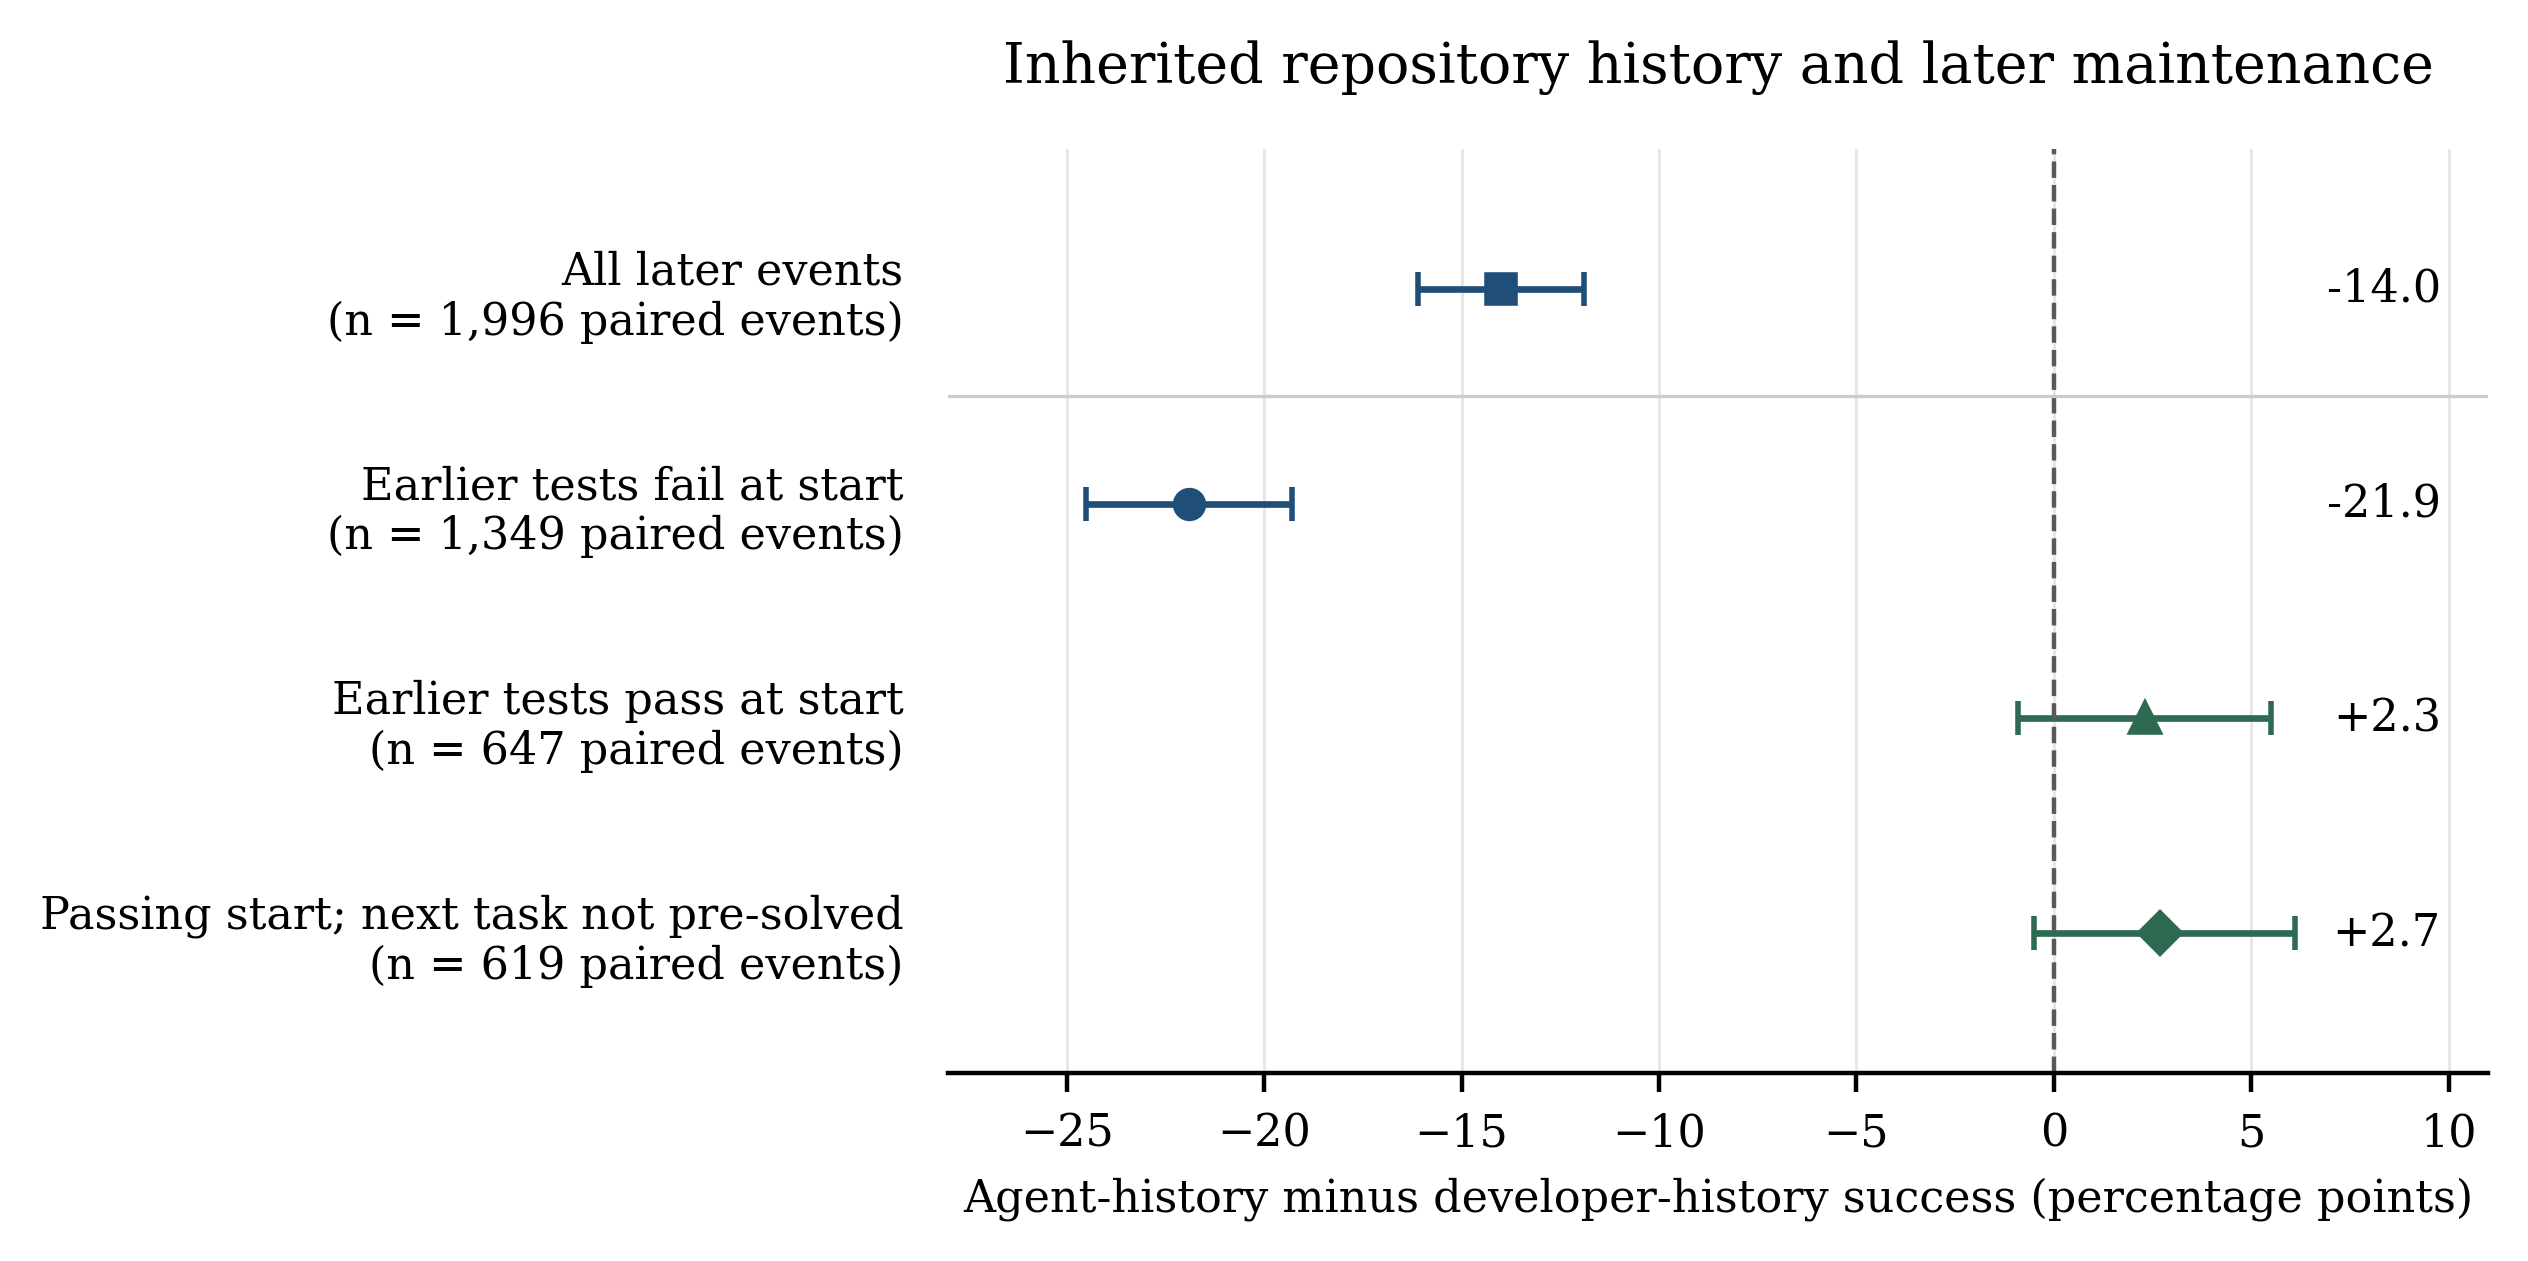
\includegraphics[width=\linewidth]{fig-inherited-history.png}
\caption{Later maintenance from two repository histories. Points and 95\%
repository-clustered bootstrap intervals are transcribed from Pan et~al.,
Table~3~\cite{pan2026swemaintain}. The outcome is event resolution: current
and all earlier non-superseded hidden tests pass. Negative differences favour
developer history. The 1,996 paired events come from 100 three-event episodes
in 50 Python repositories, evaluated with five systems and two models.
Subgroups overlap and are selected by the agent-history starting state;
the last excludes pre-solved and unevaluable tasks. They are not randomised
repair conditions.}\label{fig:inheritedhistory}
\end{figure}

The conversation and repository studies therefore locate two different
transmission pathways. Resetting context addresses the first, but not faulty
code retained for the next feature. SlopCodeBench and SWE-CI extend the
evaluation horizon to iterative structural erosion and behavioural
regressions~\cite{orlanski2026slopcodebench,chen2026sweci}. A maintainability
study using late-2024 coding assistants found no significant downstream
difference; only its second phase was randomised
~\cite{borg2025echoes}. This is assistant-era evidence, not a test of the
current autonomous agents. The emerging
question is which inherited failures survive, how they affect later work,
and which interventions prevent or repair them.

\paragraph{Output and review capacity.}
Understanding changes
is a major challenge of code review; habituation, fragmented context and
uneven retrieval from long contexts may limit scrutiny as output
grows~\cite{bacchelli2013review,yu2026habituation,cemri2025multiagent,liu2024lost,hong2025contextrot}.
Faster feature delivery also shortens the time available to discover that an
earlier assumption has become the foundation of another change. Further
empirical and practitioner context is retained in the ancillary supplement.

\subsection{Corrective instructions as maintenance debt}\label{sec:instructiondebt}

A failed agent action often invites a new instruction: run this check, never
edit that file, remember this exception. GitHub's account of more than
2,500 agent-definition files recommends starting small, testing and adding
detail when an agent makes mistakes~\cite{nigh2025agentsmd}. The resulting
guidance can preserve useful lessons, but it also becomes another maintained
system. Chatlatanagulchai et~al. document ongoing maintenance of this
material~\cite[Secs.~4.2.2--4.2.3]{chatlatanagulchai2026readmes}.
Here \emph{instruction debt} denotes the avoidable burden of obsolete,
duplicated, conflicting or poorly routed directives in prompts, skills and
handover notes. This extends the maintenance question from the product to
the machinery that changes it.

Repository histories show that this material evolves. Mohsenimofidi et~al.
found no post-creation change in 77 of 155 instruction files. In the ten most
frequently changed files, however, they classified 169 commits: 78 added
instructions, 59 modified them and 23 removed them. These are three of nine
categories, with 242 assignments in total, rather than a partition of the
169 commits~\cite[Sec.~4.3, Table~2]{mohsenimofidi2026context}.
Chatlatanagulchai et~al.'s manual analysis of 100 post-adoption commits
produced 78 addition, 32 modification and 19 deletion labels; addition labels
occurred across 66 distinct commits. Figure~\ref{fig:instructionmaintenance}
replots the label counts~\cite[Secs.~4.2.2--4.2.3]{chatlatanagulchai2026readmes}.
These histories contain accumulation and pruning, rather than a uniform
march towards longer files. The authors associate their day-scale edit
intervals with ongoing project maintenance rather than immediate prompt
debugging.

\begin{figure}[!htbp]
\centering
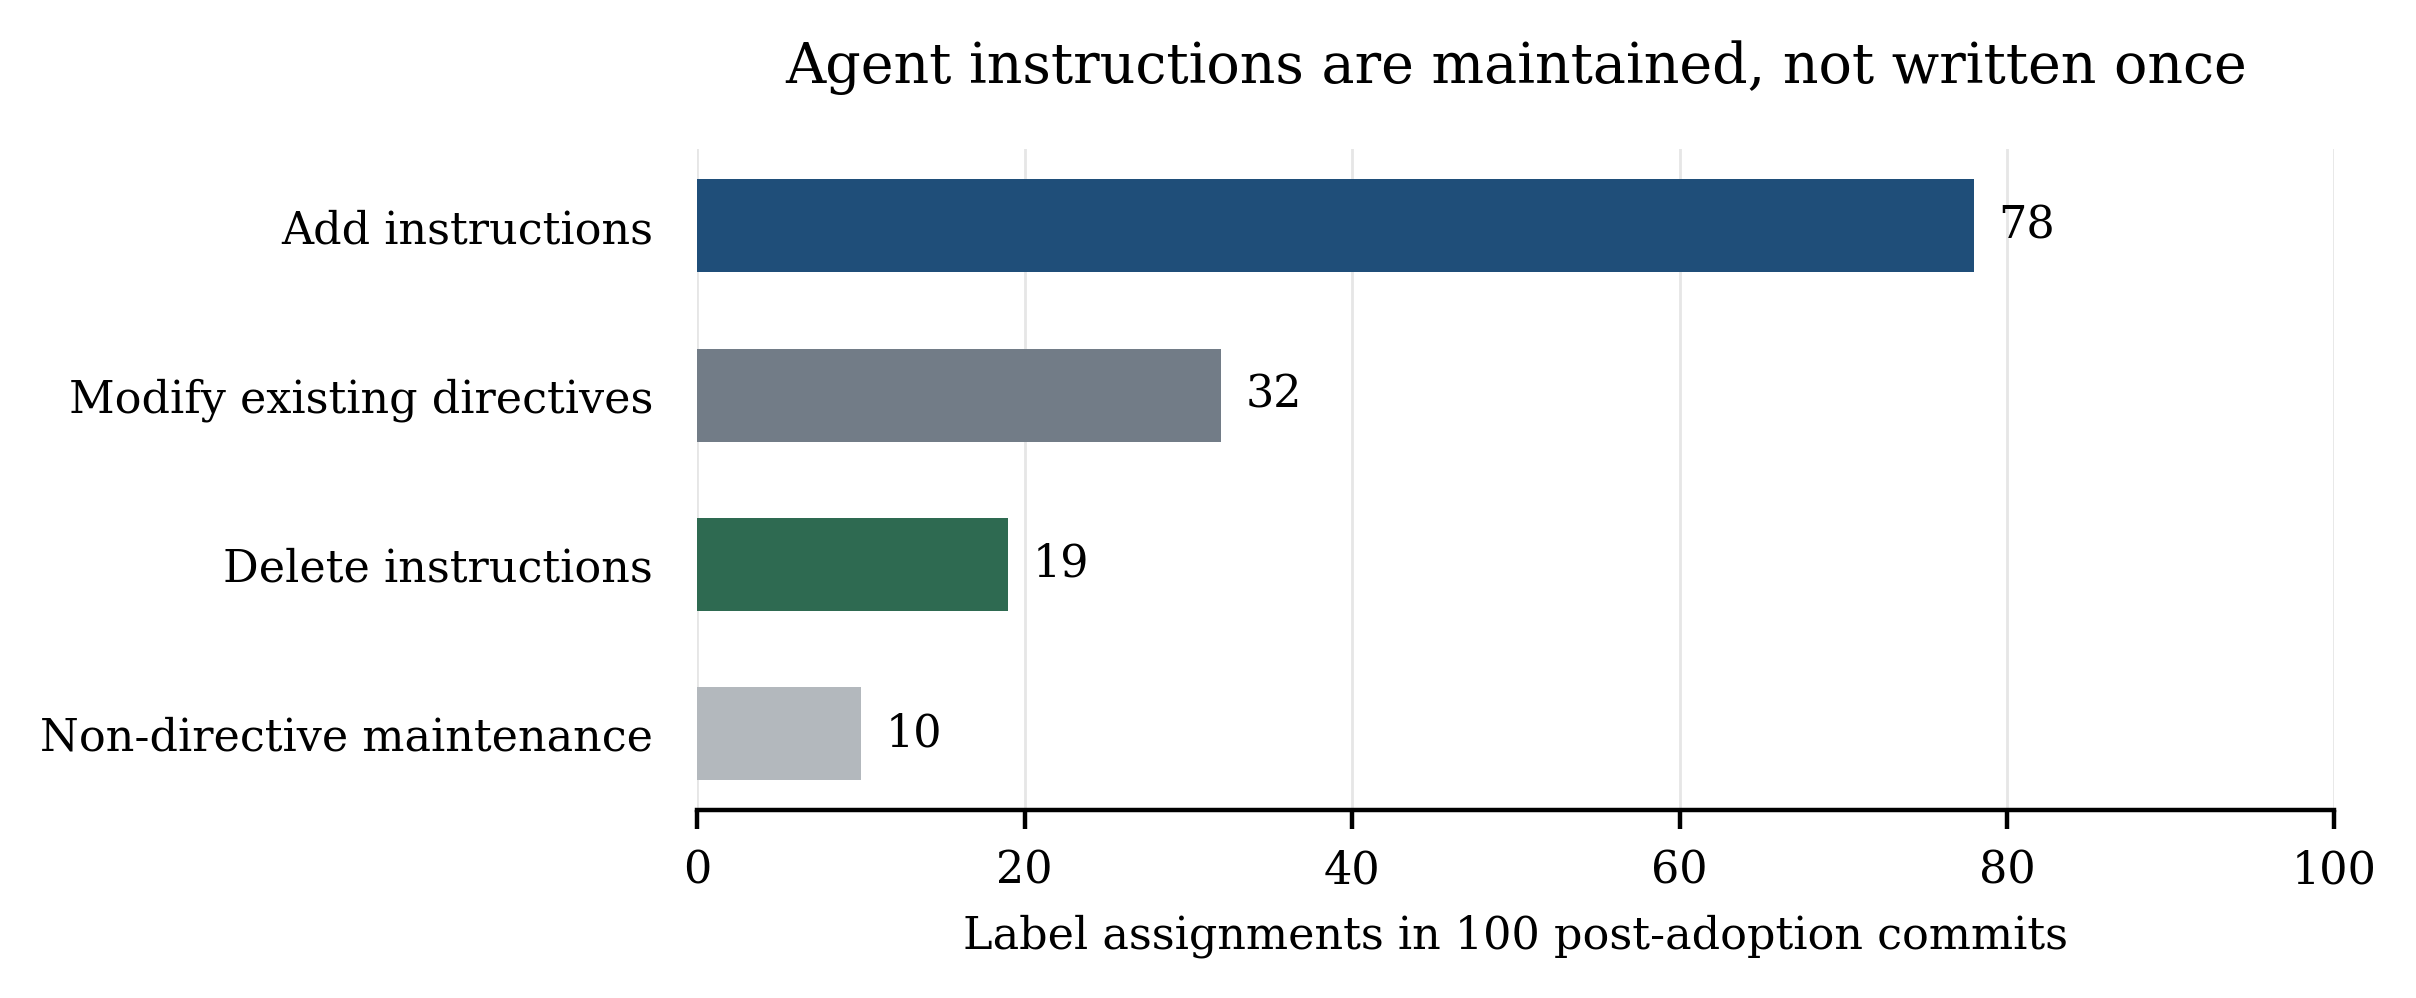
\includegraphics[width=0.94\linewidth]{fig-instruction-maintenance.png}
\caption{Instruction-file maintenance in 100 randomly sampled post-adoption
commits, from Chatlatanagulchai et~al., Sections~4.2.2--4.2.3
\cite{chatlatanagulchai2026readmes}. Commits can receive several labels;
line-level and section-level add/delete labels are combined. The ten
non-directive maintenance labels are the remainder of 139 total assignments.
The chart counts edit types, not net token growth or effects on agent
performance.}\label{fig:instructionmaintenance}
\end{figure}

Gloaguen et~al. test the effect of supplying such context. Across four
agent--model pairings on 300 SWE-bench Lite tasks and 138 CTXbench tasks,
LLM-generated context files increased average inference cost by 20\% and
23\%, respectively; task success was slightly lower, by 0.5 and 2 percentage
points, without significant differences from the no-file baseline.
Developer-written files performed significantly better than LLM-written
files on CTXbench ($p=0.038$). Agents followed the instructions, performed more testing
and exploration, and spent more reasoning tokens. Yet file length did not
explain success, and generated context helped when other documentation was
removed~\cite[Secs.~4.2--4.4, App.~B]{gloaguen2026agentsmd}.
Instruction count and loaded tokens are therefore different exposures from
the obligations and behaviours those instructions induce.

Anthropic's context-engineering account describes the practical tension:
provide enough information to guide action, but avoid brittle prompt logic
and an expanding catalogue of exceptions~\cite{rajasekaran2025context}.
Maintaining these instructions means preserving necessary constraints while
replacing accumulated exceptions with coherent rules, executable checks and
task-specific retrieval. To test the corrective-rule
spiral directly would require versioned instructions, actual session inputs
and outcomes across successive revisions. The testbed record supplies document
growth and rule changes; the consolidation protocol tests a bounded form of
handover maintenance by replacing, rather than appending to, its design note.

SkillOpt supplies counterevidence to treating instruction change as
inherently harmful. Its first-party account describes bounded edits to
skill files, held-out validation and retention of successful versions
without changing the target model's weights~\cite{microsoft2026skillopt}.
Procedural knowledge needs evaluation and maintenance; its length alone
tells us little about its quality.

Jiang et~al.'s preprint compares workflow memory with skills distilled from
the same execution histories. Its paired trajectory analysis associates
skills chiefly with more reliable procedures, while also identifying
misapplication and insufficient runtime verification
\cite[Secs.~3.3, 5.1--5.3]{jiang2026skills}.
This qualifies an instruction-debt account: retained guidance can stabilise
execution rather than merely burden context. Their retrieval study also
separates skill access from task success; in their comparison, lower
exact-match access was observed alongside sustained downstream success
\cite[Sec.~5.5]{jiang2026skills}. Because retrieval diagnostics are run
separately from task execution, this comparison does not isolate the effect
of reduced skill access. Neither result measures the effects of
accumulating repository instructions across feature changes.

\subsection{Refactoring, review and evaluation boundaries}\label{sec:evaluationwork}

Agentic refactoring, review and human correction are already studied.
RefactorBench evaluates 100 handcrafted multi-file refactoring tasks across
nine Python repositories, not scheduled consolidation between feature
additions~\cite{gautam2025refactorbench}. Kumar et~al.'s ASE~2025 study
observed developers collaborating with agents on existing issues: incremental,
active collaboration was associated with greater success, not randomly
assigned to establish an optimal intervention rate~\cite{kumar2025agents}.
SWE-Sharp-Bench supplies a reproducible C\# issue-resolution benchmark and
curation pipeline~\cite{mhatre2025swesharp}; reproducible repository-scale
evaluation itself is not a contribution claimed here.

Two recent preprints sharpen the evaluation problem. CRBugBench evaluates
review agents on 1,000 open-source and 800 proprietary tasks from one company,
reporting weaker detection on complex, non-local and proprietary-context
changes~\cite{yang2026crbugbench}. It is a 9~October 2026 preprint, not an
independently replicated result establishing that review cannot work.
\emph{Building to the Test} reports near-perfect behavioural scores for demos
while the requested reusable library was unused or absent in seven of
twelve oracle-in-the-loop runs. Its unchanged,
source-hidden oracle did not check that delivery contract~\cite{ma2026building}.
This is distinct from altering tests, as examined in
ImpossibleBench~\cite{zhong2026impossiblebench}: test integrity and adequate
outcome coverage are separate safeguards.

These studies narrow the proposed novelty to the case trace and the specific
prospective package comparison, including an unforeseen change request. They
also caution against assuming that another reviewer, a stricter check or a
high hidden-test score necessarily certifies the intended deliverable.
Preprints, observational
studies, practitioner accounts and first-party industrial reports have different
evidential roles; none substitutes for the planned controlled comparison.
AgentRx's first-party release describes evidence-backed diagnosis of a
trajectory's first critical failure~\cite{microsoft2026agentrx}. It motivates
traceable failure localisation. An independent diagnosis of the AMA mechanisms
remains outstanding.

\subsection{Optimisation with behavioural feedback}\label{sec:factory}

Pavlenko et~al.'s \emph{Towards an AI Software Factory for Data Systems}
offers a complementary case~\cite{pavlenko2026factory}. Hotspan packages
optimisation targets from telemetry, analysis and reviews; Darwin explores
candidate changes through code--test--debug--reflect cycles. The setting is
existing, human-architected systems with stable semantics and measurable
objectives such as latency. Reported optimisation gains are evidence against
treating high agent throughput as inherently unproductive, not a controlled
estimate of end-to-end productivity, general maintainability or future
changeability. Their application-work productivity calculation excludes
infrastructure and onboarding time, and output enters engineering review.
The work establishes a precedent for bounded agent-led correction; it does
not isolate consolidation between feature additions or product-goal selection.

\subsection{The practitioner conversation}\label{sec:practitioners}

Waseem et~al. describe rapid generation alongside architectural inconsistency,
security concerns and maintenance overhead~\cite{waseem2025vibe}. That trade-off
is not claimed as new here; the contribution is the case trace and prospective
package comparison.

Beck supplies the conceptual bridge: augmented coding retains care for code,
complexity and tests; alternating features with consolidation aims to restore
options consumed by additions~\cite{beck2025augmented,beck2026prodacity,beck2025devslow}.
Understanding and abstraction are distinct from producing more
artefacts~\cite{beck2026mathematicians}; learning through working software
is developed in Beck's talk~\cite{beck2026prodacity}. These arguments motivate testing
bounded reflective work, not an established remedy or a permanent human--agent
boundary. Extended practitioner accounts remain in the ancillary supplement.

Spec-driven development adds structure, but not an automatic outcome oracle.
Spec Kit proposes specification, planning, tasks and implementation;
B\"ockeler describes both ignored and over-followed instructions; and a study
of practice reports reliability benefits alongside planning and review
costs~\cite{delimarsky2025speckit,boeckeler2025sdd,agarwal2026sdd}.

\subsection{Engineering principles behind consolidation}\label{sec:theory}

The engineering lineage is more specific than a general call for better
code. Beck links small structural changes to test feedback
\cite{beck2002tdd,beck2023tidy}; Gamma, Helm, Johnson and Vlissides describe
reusable designs with explicit applicability, consequences and trade-offs
\cite{gamma1995patterns}. Martin emphasises executable technical feedback
\cite{martin2026productengineers}, while Fowler's design stamina hypothesis
connects attention to design with the cost of later features
\cite{fowler2007stamina}. These ideas motivate the consolidation checklist:
locate responsibilities, expose dependencies, preserve contracts and leave
a concise account of design choices. They are design rationales, not
empirical evidence that the proposed agent intervention is effective.
Applying more named patterns is not itself an outcome; retained behaviour
and the cost of subsequent change are the proposed tests.

Naur distinguishes a programmer's theory of the system from its documentary
record; Brooks locates essential difficulty in the conceptual construct,
not its representation~\cite{naur1985theory,brooks1987silver}. Royce and Gall
motivate early experience of working behaviour~\cite{royce1970,gall1975}.
XP's short releases and tests~\cite{beck2004xp,beck2002tdd}, Crystal Clear's
incremental team practice~\cite{cockburn2004crystal}, tracer
bullets~\cite{hunt1999pragmatic} and Agile's preference for working
software~\cite{agile2001manifesto} make that feedback concrete.
Small reversible structural changes supply a consolidation
practice~\cite{beck2023tidy}.

Automation can shift effort from producing to monitoring and intervention,
with substantial metacognitive demands~\cite{bainbridge1983ironies,simkute2024ironies,tankelevitch2024metacognitive}.
Associations between confidence in AI and reduced scrutiny do not establish
causation~\cite{lee2025critical}. Goodhart and Strathern motivate checking
completion proxies against their intended outcomes~\cite{goodhart1975,strathern1997improving}.

\subsection{Hypervelocity Engineering (HVE Core)}\label{sec:hve}

HVE Core is an open-source framework from Microsoft that supplies workflow
structure for GitHub Copilot; the author's coordinator provided autonomous worker dispatch.
Its Research, Plan, Implement and Review (RPI) workflow leaves dated records
under \texttt{.copilot-tracking}, with explicit human stops and review.
The case used those file-based handovers and its Experiment Designer's Minimum
Viable Experiment method~\cite{hvecore}; the coordinator supplied the
separate autonomous delivery loop. Framework product details are secondary
context, retained in the ancillary supplement.
The author reports using HVE Core plugin snapshot \texttt{plugins-v3.3.106} throughout the
case. Its snapshot commit is
\texttt{2df5013e29ebfd2ce61bcd0cf021d8c8186482eb}, generated from source commit
\texttt{e9af018fe5ffbfbc72321a8bca21fb987359af08}. Historical use is an author account;
the snapshot identifiers do not establish an installation date.

% ===========================================================================
